\documentclass[a4paper,11pt,report,dvipdfmx,uplatex]{jsbook}
\usepackage{lllsdepp}

% ===== 注意 =====
% このファイルのプリアンブルには \usepackage を書かないでください
% lllsdepp.sty を直接編集するようにしてください

% ===== 執筆者記入事項 ここから=====
\thesisNendo{201x}	% 提出年度
\thesisClass% 所属 下記2行のうち当てはまる方をコメントイン
% {教育学部}	% 卒業論文
{教育学研究科}	% 修士論文
\thesisAuthor{本郷 弥生}	% あなたのお名前(姓名は全角スペースで分ける)
\thesisAuthorID{23-000000}	% あなたの学籍番号(半角)
\thesisTitle{教育学研究科・教育学部学位論文執筆要綱}	% 論文題目
% サブタイトルがなければ下の行をコメントアウト
\thesisSubTitle{生涯学習基盤経営コース・教育実践政策学コース向け}	% サブタイトル(ダッシュなし)
\thesisTeacher{浅野 柏子 教授}	% 姓[半角スペース]名[全角スペース]職階
% ===== 執筆者記入事項 ここまで =====

\begin{document}

% ===== 表紙の出力 =====
\maketitle

% ===== 目次 =====
\frontmatter	% 目次に独自のページ番号を与える
\setcounter{tocdepth}{3}
\tableofcontents % 章節目次
\makeatletter
	% 修士論文ならば図表目次を出力
	\ifthenelse{\equal{\@thesisClass}{教育学研究科}}{
		\listoffigures	% 図目次
		\listoftables	 % 表目次
	}{}
\makeatother


% ===== 本文 =====
\mainmatter	% 本文の開始を宣言し、ページ番号を振り直す
%! TEX root = ../thesis_main_sample.tex

\chapter{体裁ガイドライン}
	\label{chp:guideline}

	本文書は、東京大学教育学研究科生涯学習基盤経営コース及び同教育学部教育実践政策学コースの所属学生が執筆する学位論文の執筆スタイルを規定するものである。
	以下、断りが無ければ「本コース」を上記2コースの総称とする。
	本章でスタイルの詳細について記述し、次章では本文書の生成に用いたテンプレートファイルについて述べる。

	\section{言語}
		\label{sub:language}

		執筆に用いる言語は日本語または英語とする。
		ただし、教育学研究科修士論文要旨及び教育学部卒業論文要旨は必ず日本語で書くことになっている。
		以下、本節で説明するスタイルは日本語での執筆を対象とする。
		英語で執筆する際は、研究対象の領域に最も近い学術雑誌のスタイルガイドを選び、準拠すること。
		その際、準拠したスタイルガイドは学位論文中に明記せよ。

	\section{製本上の構成}
		\label{sub:seihon}

		本コースの学位論文はA4用紙に印刷し、左綴じで製本のうえ提出すること。
		このとき枚数が少なすぎると安定しないので,100ページ以内であれば片面印刷するとよい。
		その他、本コースにおける製本の規定及び実践的なアドバイスについては\cref{app:seihon}で案内があるので参照されたい。
		学位論文の中身は次の順番で製本すること。

	\begin{itemize}
		\item 表題紙
		\item 目次
		\item 本文
	\end{itemize}

	以上の構成要素の詳細については\cref{sec:layout}以下を見よ。
	卒業論文は本文が20枚以上であることが要件である
	\footnote{修士論文には枚数規定はない。}。

	\section{全体のレイアウトと字体}
		\label{sec:layout}

		以下はテンプレートを適切に利用すれば自動的に適用される。

		\subsection{レイアウト}
			\label{sub:layout}

			\subsubsection{表題紙}
				\label{subs:titlepage}

				提出年度と学位論文の種類(修士論文または卒業論文)を上余白40mm以上とって配置し、そこから45mm程度を空けて論文題目(サブタイトル含む)を置くこと。
				下余白30mm程度の位置に、自身の所属(大学・大学院名、学部・研究科名、学科・専攻名、コース名)、学籍番号、氏名、指導教員名・職名を記述せよ。
				文字は全て中央揃えとする。
				表題紙にはページ番号を振らない。

			\subsubsection{目次}
				\label{subs:tableof}

				表題紙に続けて、本文の章節目次を作成する。
				目次タイトルと目次本体があれば、後者のレイアウトは1段組である限りにおいて自由とする。
				図表を含むときは図目次、表目次の順に追記するようにせよ。
				このとき、各目次は改ページしたうえで連結すること。
				また、目次にはローマ数字(i, ii, iii, \dots)など本文と異なる数字を用いて独自のページ番号を振るようにする。
				ページ番号の場所は本文(\cref{subs:body})に同じ。

			\subsubsection{本文}
				\label{subs:body}

				本文は1段組で構成し、文字数は1行45字程度、行数は35行程度とする。
				余白は左右25mm、上下30mm程度をとること。
				ヘッダーとフッターを考慮しても、本文と上下の余白が40mm以上離れていればよい。
				本文が100ページを超えて両面印刷にて製本する場合、奇数ページ・偶数ページごとに左右の余白を変えてもよい。

				\paragraph{ヘッダー・フッター}
					\label{subs:header_footer}

					フッター中央にはページ番号のみを配置し、原則としてヘッダーには何も書かないものとする。
					各節が十分に長いために読者が道に迷う可能性があるとの懸念にしたがって、可読性のために章節タイトルを表示するなどの運用は可とする。


		\subsection{書体・書式・文字サイズ}
			\label{sub:font}

			本コースの学位論文の、文字から構成される要素は\cref{tab:font}に示す書体・書式・文字サイズを用いよ。
			ただし、表題紙について、年度と学位論文の種類は項タイトル、
			所属・指導教員・学籍番号・氏名・指導教員は本文と同じとする。
			また、小項以下の項目立てを用いる場合には項タイトルと同じくし、頭に記号を用いるなどして項タイトルと差異化せよ。

			\begin{table}[tb]
				\caption{文字から構成される論文上の要素に用いるべき書体・書式・文字サイズ}
				\label{tab:font}
				\centering

				\begin{tabular}{lccc}
				\toprule
				\textbf{構成要素} & \textbf{書体} & \textbf{書式} & \textbf{文字サイズ}\\
				\midrule
					論文題目 & 明朝体 & 立体 & 18pt \\
					サブタイトル & 明朝体 & 立体 & 14pt \\
					章タイトル & ゴシック体 & 太字 & 20pt \\
					節タイトル & ゴシック体 & 太字 & 14pt \\
					項タイトル & ゴシック体 & 太字 & 12pt \\
					本文 & 明朝体 & 立体 & 20pt \\
				\bottomrule
				\end{tabular}
			\end{table}

	\section{本文の構造化方法}
		\label{sec:structure}

		本文の構造は以下の順とする。

		\begin{enumerate}
			\item 各章(注は脚注として内包)
			\item 謝辞
			\item 参考文献
			\item 付録
		\end{enumerate}

		各章の内部は、論理的に章・節・項の3階層に収まるのが構成のわかりやすさと読みやすさの観点から望ましい。
		節・項の番号付けはハーバード方式(2.3.1のような形式)とする。
		小項以下は箇条書きなどで適宜代用し、目次への記号の反映は任意とする。

		付録と謝辞は章と同等の扱いとするが、付録にはアルファベット大文字で「付録A」などと番号付けする一方、謝辞には章番号をつけないものとする。
		参考文献の詳細はあとで述べる。

	\section{本文の表記方法}
		\label{sec:writing_manner}

		\paragraph{句読点}
			\label{par:punct}

			和文は句点を全角コンマ(,),読点を全角読点(。)とする。
			欧文中では半角のコンマ (,)とピリオド (.) を用い、半角スペースを後置する。
			また和文中に欧文の句を挿入する際には、半角スペース相当の空白を入れること
			\footnote{WordでもLaTeXでも自動で入る}。

		\paragraph{強調}
			\label{par:inline_markup}

			文章の一部、単語や句を強調したい場合、和文には\emph{太字}のみを用い、斜体は使わないようにせよ。
			このとき太字はゴシック体にするのが望ましいが,統一されている限りにおいて明朝体でもよい。
			読みにくくなるため、引用文で用いられている以外は下線,圏点の利用は控える。

			一方、欧文の強調はセリフ体の斜体を基本的に用いることとし,太字・ゴシック・下線の利用は控える。
			ただし、強調したい和文キーワードの一部に欧文が含まれる場合は、和文と揃えて太字にする(例:\textbf{MARCフォーマット})。

			以上において控えるべきとした強調方法については、強調部分のなかでさらにその一部を強調したい場合であれば利用してよいものとする。

		\paragraph{図表}
			\label{par:fig_tab}

			図表は任意の位置に置いてよいが、図表番号及びキャプションを必ず付与すること。
			ただしその位置は、表については上に、図については下に付与するものとする(e.g., \cref{tab:font,fig:sample})。
			図表番号はハーバード方式に従っても、全体を通して連番としてもよい(本要綱では前者とした)。

			\begin{figure}[tb]
				\centering
				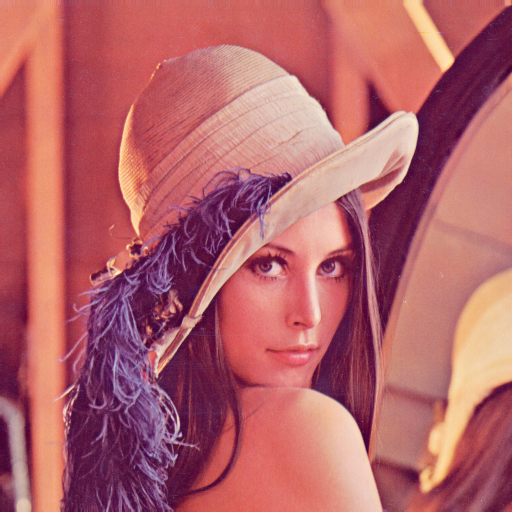
\includegraphics[width=5cm]{figure/Lenna.png}
				\caption{サンプル画像として著名な Lenna Sjööblom さん}
				\label{fig:sample}
			\end{figure}

		\paragraph{記号}
			\label{par:symbol}

			本文中でよく使われる一方で誤用の多い記号類について注意点を述べる。

			\begin{description}
				\item[二重かぎかっこ(『, 』)] 和文書籍の書名を表すときに用いよ。英語と違って太字にしないこと。
				\item[丸かっこ((, ))] 欧文中で丸かっこを使うときはその前後にスペースを入れることに注意せよ。また、和文を内包させる場合は全角にする。
			\end{description}

			\noindent
			その他、とくに欧文(英語)環境における正しい記号の使い方は \texttt{english punctuation} などのキーワードでweb検索するとよい。

		\paragraph{引用}
			\label{par:cite}

			参考文献の一部を文字通り引用する場合、本文中に埋め込む方式(inline quote)とパラグラフとして分離する方式(block quote)の2つがある。
			inline quote であるが、次に示すようにかぎかっこ(「, 」)で引用部分を囲み、文中に埋め込めばよい。
			ただし引用文中にもかぎかっこがある場合は、二重かぎかっこ(『, 』)に変更すること
			\footnote{引用文がさらに2重かぎかっこを含む場合はかぎかっこに変更する。}。

			\begin{itembox}[l]{Inline quote}
				澤田昭夫は良い論文について \textcquote[p. 19]{sawada}{よい論文は統一unity,連関coherence,展開developmentにおいて優れた論文あるいは明確性clarityにおいて優れた論文}だとしている。
			\end{itembox}

			\noindent
			次に block quote であるが、次のように前後と左側に余白を与えるようにする。
			3行以上になるようであれば block quote を使うようにするとよい。

			\begin{displaycquote}[p. 74]{sawada}
				論文書きでもっとも大切なのは,問を疑問文の形で切り出すことで,それがレトリックで言う発見・構想です。
				もっとも大切だというのは,それができればつまり全体を貫く主な問が何であるかを確定することができれば,論文の首尾一貫性,統一性を保証する基本的条件が整ったことになるからです。

				そのつぎに大切なのは,論文の構成,材料の配置です。
				その際,肝に銘じなければならないのは,構成・配置の大原則は起承転結ではなく,序・本・結(序と本論と結び)だということです。
			\end{displaycquote}

			\noindent
			いずれも引用元の参考文献と、当該引用文が記載された箇所(ページ番号など)を引用の末尾に明示すること。
			その記述方法は\cref{sub:ref_style}と同様である。


	\section{参考文献スタイル}
		\label{sec:bib_style}

		本説では、本文中で参考文献を示すときの参照方法と文献リストの記述法を述べる。

		\subsection{参照方法}
			\label{sub:ref_style}

			基本的には主語として「著者 (年)」とするか、文末に「(著者, 年)」を置く \emph{author-year} 形式が望ましいが、一貫している限りにおいて \emph{number} 形式(参考文献に番号を振り、「[1]」のように参照する)も可とする。

		\subsection{文献リストの記述方法}
			\label{sub:ref_list_sylte}

			基本的には、本項で紹介するスタイルを採用せよ。
			ただし論文全編にわたって一貫している限りにおいて、各自の研究領域に最も近いスタイルを使っても良い
			\footnote{例えば本テンプレートの参考文献リストは日本経済学会に準拠している}。
			その際は指導教員やその指導を受けている先輩の院生に確認すること。
			リストに記載する文献の順番は「著者順」または「(本文での)引用順」のいずれかとする。

			% 参考文献リストの書式の乱れは研究姿勢の乱れであることを自覚するように

		\subsubsection{図書の場合}

			\begin{description}
				\item[和:] 著編者名 『書名』 \{版表示,\} \{出版地,\} 出版社, 出版年, \{総ページ数,\} 当該部分のページ.
				\item[洋:] author. \textit{title}. \{edition,\} place of publication, publisher, year, \{total page,\} page.
			\end{description}

			\begin{screen} \begin{itemize}
				\item 近藤二郎 『社会科学のための数学入門』 東京経済新報社, 1973,
				p. 37--40.

				\item Barzun, Jacques and Graff, H. F. \textit{The Modern Researcher.}
				Rev. ed., \\New York, Harcourt, 1970, p. 165.
			\end{itemize} \end{screen}


		\subsubsection{翻訳書の場合}

			\begin{description}
				\item[和:] 著編者名 『書名』[原書名(イタリックで記載) \{版表示,\}
				\{出版地, \} 出版社, 出版年,] 翻訳者名, 出版社, 出版年, \{総ページ数,\} 当該部分のページ.
				\item[洋:] author. \textit{title of translation} [\textit{original title}. \{edition,\} place of publication, publisher, year,] name of translator, place of publication, publisher, year, \{total page,\} page.
			\end{description}

			\begin{screen} \begin{itemize}
				\item Varles, Jana ed. 『情報の要求と探索』 [\textit{Information Seeking:
				 Basing Services on User's Behaviors.} North Calolina,
				 McFarland \& Company, 1987] 池谷のぞみ,	 市古健次, 白石英理子, 田村俊作訳,
				 勁草書房, 1993, p. 10.

				\item Schneider, Georg. \textit{Theory and History of Bibliography.}
				 [\textit{Handbuch der Bibliographie.} e Aufl., Berlin, Knopt, 1978,]
				 tr. by R. R. Shaw, New York, Columbia University Press, 1934, p. 14--15.
			\end{itemize} \end{screen}

		\subsubsection{編集書の一部(図書形態の論文集の一論文を含む)の場合}

			\begin{description}
				\item[和:] 当該部分の執筆者名 ``当該部分の題名'' $<$編者名 『書名』 \{版表示,\} \{出版地,\} 出版社, 出版年$>$ \{総ページ数,\} 当該部分のページ.
				\item[洋:] author. ``\textit{title}''. $<$editor. \textit{book title}, \{edition,\} place of publication, publisher, year$>$ \{total page,\} page.
			\end{description}

			\begin{screen} \begin{itemize}
				\item 宮坂広作 ``余暇と社会教育'' $<$碓井正久編著 『社会教育』 第一法規, 1970$>$ p. 201--203.

				\item Groom, Geofrey. ``Bibliography of older material'' $<$Garvin, L. H. ed. \textit{Printed Reference Material.} 2nd ed., London, Library Association, 1984$>$ p. 456--501.
			\end{itemize} \end{screen}


		\subsubsection{逐次刊行物掲載記事(雑誌論文を含む)の場合}

			\begin{description}
				\item[和:] 執筆者名 ``論題名'' 『掲載逐次刊行物名』 vol. XX, \{no. XX,\} 発行年\{月\}, 当該部分のページ.
				\item[洋:] author. ``\textit{title},'' \textit{name of periodical}, vol. XX, \{no. xx,\} year\{month\}, page.
			\end{description}

			\begin{screen} \begin{itemize}
				\item 小野寺夏生 ```Bibliostatistics': 情報現象の統計学的説明'' 『情報管理』
				vol. 21, no. 10, 1979, p. 782--802.

				\item 小野寺夏生, 中井浩 ``単純なモデルからのZipfの法則の導入'' 『情報科学技術
				研究集会論文集』 vol. 33, no. 3, 1977, p. 129--138.

				\item Brookes, Bertram C. ``Theory of the Bradford Laws,'' \textit{Journal of
				Documentation,} vol. 33, no. 3, 1977, p. 180--209.

				\item Nelson, Micheal J. and Tague, Jean M. ``Sprit Size-Rank Models for the
				Distribution of Index Terms,'' \textit{Journal of the American Society
				for Information Science,} vol. 36, no. 5, 1985, p. 283--296.
			\end{itemize} \end{screen}

		\subsubsection{Web上のリソース}

			web上のリソースについては,書誌情報の最後に ``入手先URL (アクセス日)''
			(``available from (URI), (accessed date)'') を記入する。
			それ以外の項目は図書並びに逐次刊行物掲載記事の規定に準じ,入手先の情報から明らかである項目を記述せよ。

			\begin{screen}
				 情報メディア学会 ``『情報メディア研究』への各種原稿の投稿について'' http://www.jsims.jp/toko.html (アクセス日: 2008/10/27)
			\end{screen}

%!TEX root = ../thesis_main_sample.tex

\chapter{テンプレート使用方法}
	\label{chp:readme}

	\section{ファイル構成}
		\label{sec:contents}

		本テンプレートは下記のような構成となっている。

		\begin{itemize}
			\ttfamily
			\item thesis\_guideline.pdf: この要綱のファイル
			\item \textbf{LaTeX/}
			\begin{itemize}
				\item thesis\_main.tex: このファイルに自分の論文を書く
				\item thesis\_main\_sample.tex: この要綱の tex ソースファイル(参考・\TeX{} 環境のテスト用)
				\item sample\_bibliography.bib: この要綱で用いたBibTeXによる参考文献リストファイル
				\item jecon\_custom.bst: BibTeX用の参考文献スタイルファイル
				\item latexmkrc: latexmkによる自動コンパイルの設定ファイル
				\item lllsdepp.sty: この要綱のスタイルファイル
				\item \textbf{figure/}: 画像ファイルの格納場所
					\begin{itemize}
						\item Lenna.png: サンプル画像(\cref{fig:sample})
					\end{itemize}
				\item \textbf{body/}: 本文のtexソースを置く場所
					\begin{itemize}
						\item sample\_guideline.tex: \cref{chp:guideline} のソースファイル
						\item sample\_usage.tex: \cref{chp:readme}のソースファイル
					\end{itemize}
				\item \textbf{appendix/}: 付録のtexソースを置く場所
					\begin{itemize}
						\item sample\_appendix.tex
					\end{itemize}
			\end{itemize}
			\item \textbf{Office/}: Officeソフトウェア向けテンプレート集
				\begin{itemize}
					\item msword\_template-master.docx: Word\textsuperscript{\textregistered}を用いる場合はこのファイルに執筆(修士論文用)
					\item msword\_template-bachelor.docx: Word\textsuperscript{\textregistered}を用いる場合はこのファイルに執筆(卒業論文用)
					\item libreoffice\_template-master.docx: LibreOffice を用いる場合はこのファイルに執筆(修士論文用)
					\item libreoffice\_template-bachelor.docx: LibreOffice を用いる場合はこのファイルに執筆(卒業論文用)
				\end{itemize}
		\end{itemize}

		\noindent
		執筆に用いるソフトウェアに応じて、\LaTeX{} 版か Office 版を選択せよ。
		以下の節では、それぞれのフォーマットについて、その使い方を説明する。

	\section{LaTeX}
		\label{sec:latex}

		本テンプレートファイルは \texttt{TeXLive} の2016以降のバージョンに対応している。
		以下、使用するOSに応じた最新の \texttt{TeXLive} をインストールしている前提を置く。
		また、基本的な使用方法については理解しているものとする。

		本テンプレートは、\texttt{thesis\_main.tex}を論文の骨格の記述に用い、章ごとに分割された tex ソースファイルを本文(\texttt{body})と付録(\texttt{appendix})で区別して管理する構成となっている。

		\subsection{スタイルファイル}
			\label{sub:style_file}

			\texttt{lllsdepp.sty}が\cref{chp:guideline}で指定した体裁を再現する。
			すでに多数のマクロ・パッケージが読み込まれている状態であるが、執筆において使用したいマクロ・パッケージがある場合はこの\texttt{lllsdepp.sty}の該当箇所において直接宣言してほしい。
			\texttt{thesis\_main.tex}のプリアンブルで \texttt{\textbackslash usepackage}によるパッケージ読み込みは避けること。
			これは本テンプレートで使用している \texttt{creveref} というパッケージの制約により、\texttt{creveref}より後の行でのパッケージ読み込みが禁じられているためである。
			ただし、執筆において使用したいマクロ・パッケージの動作が、\texttt{lllsdepp.sty}にデフォルトで記述されているマクロ・パッケージの読み込み順を変更しないと保証されない場合は、この限りではない。


			% 両面印刷する場合はclassオプションからreportを外すと良い。
			% このときの左右余白やヘッダー・フッターのレイアウトは適宜変更して見やすくすること(デフォルトは汚い)。

		\subsection{メインファイル}
			\label{sub:メインファイル}

			\texttt{thesis\_main.tex}には、表紙に記入すべき情報と各章のtexソースの読み込み順を記述する。
			まず、8行目から次のような記述があるので、指示に従って執筆者自身の情報に書き換える
			\footnote{提出年度を自動化しないのは、当該年度以降に学位論文texソースをコンパイルしたときに提出年度が上書きされるのを嫌うため。}。

			\small
			\begin{verbatim}
				% ===== 執筆者記入事項 ここから =====
				\thesisNendo{201x}	% 提出年度
				\thesisClass% 所属 下記2行のうち当てはまる方をコメントイン
				% {教育学部}	% 卒業論文
				{教育学研究科}	% 修士論文
				\thesisAuthor{本郷 弥生}	% あなたのお名前(姓名は全角スペースで分ける)
				\thesisAuthorID{23-000000}	% あなたの学籍番号(半角)
				\thesisTitle{教育学研究科・教育学部学位論文執筆要綱}	% 論文題目
				% サブタイトルがなければ下の行をコメントアウト
				\thesisSubTitle{生涯学習基盤経営コース・教育実践政策学コース向け}	% サブタイトル(ダッシュなし)
				\thesisTeacher{浅野 柏子 教授}	% 姓[半角スペース]名[全角スペース]職階
				% ===== 執筆者記入事項 ここまで =====
			\end{verbatim}
			\normalsize

			各章のtexソースは、執筆者の章立てにおいて意図する順番に \texttt{\textbackslash include} コマンドで読み込む。
			章の入れ替えが楽になるほか、1つのファイルが大きくなりすぎてエディタで扱いづらくなることを防ぐ。

		\subsection{コンパイル}
			\label{sub:compile}

			本テンプレートを用いた文書は、\texttt{latexmk}を使った次のコマンドをシェル上で実行してコンパイルせよ。

			\begin{verbatim}
				$ latexmk -pvc thesis_main.tex
			\end{verbatim}

			\texttt{latexmk}は、\texttt{include/input}を用いて分散化されたtexソースの構成を追跡し、BibTeXないしMendexといった補助的に用いるコマンドを適切なタイミングで自動的に実行する\LaTeX 文書ビルドツールである。
			\texttt{pvc}オプションを与えることにより、texソースファイルの変更を逐一監視してくれるので、本文を通常通り保存するだけで種々のコンパイルが実行されるうえ、PDFビューワを開いて最新の状態を表示してくれるようになる。
			そのための設定ファイルが\texttt{latexmkrc}である。
			設定を適切に反映するために、上記のコマンドは \texttt{LaTeX/}フォルダ直下で実行すること。
			OSごとの実行コマンドの違いはこの\texttt{latexmkrc}が吸収しているので、執筆者は不具合のない限り \texttt{latexmkrc}の存在を意識する必要はない。

		\subsection{執筆}
			\label{sub:writing}

			実際の執筆において本テンプレートが推奨するコマンドを説明する。

			\subsubsection{強調}

				基本は \texttt{\textbackslash emph} を用いよ。
				これにより欧文では斜体、和文では太字が使われるようになる。
				本テンプレートのスタイルファイルでは \texttt{otf}パッケージの\texttt{bold}オプションを有効にしているため、太字はすべてゴシックになる。

			\subsubsection{引用}

				素の\LaTeX 文書においては\texttt{``\dots''}や\texttt{quote/quotation}環境が用いられるが、本テンプレートでは \texttt{csquotes} の使用を推奨している。
				スタイルファイルには既に導入されているので、inline と block それぞれで次のようにコマンドを使い分けるとよい。

				\begin{description}
					\item[Inline]  \\
						\verb|\textcquote[<ページ番号;例: p. 19>]{<引用キー;例: sawada>}{...}|
					\item[Block]  
						\begin{verbatim}
							\begin{displaycquote}[<ページ番号;例: p. 74>]{<引用キー;例: sawada>}
							    ...
							\end{displaycquote}
						\end{verbatim}
				\end{description}

				\noindent
				\texttt{text/display}と\texttt{quote}の前に一文字\texttt{c}が入っていることに注意。
				この\texttt{c}は\texttt{cite}を意味すると思うとよい。
				オプション引数(\texttt{[ ]}の中)の形でページ番号を指定すれば、自動的に引用文の後ろに参考文献情報が挿入される。

			\subsubsection{参照}

				ふつう、節や図表で付与した\verb|\label|を\verb|\ref|コマンドで参照するところ、本テンプレートでは\verb|\cref|を使うと記述が楽になる。
				この\verb|\cref|というコマンドは\texttt{cleveref}によって提供されるもので、\texttt{lllsdepp.sty}ではこれを日本語向けに設定してある。

				例えば、章番号を引用するときに通常の\verb|\ref|を用いた場合だと\verb|第\ref{chp:hoge}章|と入力しなければならないが、\texttt{cleveref}を使うと、\verb|\cref{chp:hoge}|だけで済むようになる。
				さらに\texttt{cleveref}は\verb|\label|の貼られた場所がどういう環境であるかを自動で識別し、そこが章や節であれば「第n章」、「n.m節」などと補完し、図表であれば「図n」「表m」と表示することができるので、あらゆるラベル参照を\texttt{cleveref}で代用することが出来る。


			\subsection{参考文献}
				\label{sub:bibtex}

				本テンプレートではpBibTeXを用いた参考文献処理が組み込まれている。
				したがって執筆者はBibTeX形式で参考文献リストを準備するのがよい。
				また、参考文献スタイルとしてSIST02\footurl{http://jipsti.jst.go.jp/sist/handbook/sist02_2007/main.htm}を採用している。経済学の標準的な形式を再現した \texttt{jecon}\footurl{http://shirotakeda.org/ja/tex-ja/jecon-ja.html}を元にいくつかのオプションを変更した\texttt{jecon\_custom.bst}を使用することでSIST02のサポートを実現しており、和書・洋書が混在した参考文献リストが見やすく出力されるようになっている。
				本テンプレートの\texttt{jecon\_custom.bst}は文献管理ソフトウェア \texttt{Mendeley} \footurl{https://www.mendeley.com}で出力できるBibTeX形式に準拠しており、とくに和文書籍・論文を \texttt{CiNII}\footurl{http://ci.nii.ac.jp}から \texttt{Mendeley} へとエクスポートしたときのBibTeXフォーマットにおいても著者の姓名が正しい順番に揃うように改変してある。

				したがって執筆者は \texttt{Mendeley} を用いた文献管理を行いつつ、そのデスクトップアプリケーションから出力したBibTeXファイル
				\footnote{詳しい方法は公式ドキュメントなどを参照されたい
				(\url{https://blog.mendeley.com/2011/10/25/howto-use-mendeley-to-create-citations-using-latex-and-bibtex/})。}
				を本テンプレートの\texttt{sample\_bibliography.bib}と同じ階層に置くことで、快適な参考文献処理が行えるのである。
				% TODO: should be update line number according to jecon_custom
				ただし、BibTeXファイルをその他の方法で独自に管理していて日本人著者の姓名が逆に表示される場合は、\verb|jecon_custom.bst|の168行目から始まるオプションを0に変更せよ。

	\section{Office}
		\label{sec:office}

		Officeソフトウェア向けにもテンプレートを用意した。
		対応しているソフトウェアは、Microsoft Office Word \textsuperscript{\textregistered} とLibreOffice \footurl{https://www.libreoffice.org} である。

		Word \textsuperscript{\textregistered} 版のテンプレートはファイル形式として \texttt{.doc}\textbf{x}を採用した。
		本テンプレートはOffice 2016以上のバージョンが推奨である。
		それ未満のバージョンにおけるテンプレートの動作不良は一切サポートしない。

		LibreOffice版はバージョン5.3.4で動作確認している。
		それ以上のバージョンであれば動作に大きな問題はないと考えられる。

		ただしOfficeテンプレートを使う場合は、\LaTeX{}版と違って以下の点が不便であることから、あまり推奨しない。
		執筆には\LaTeX{}版を使うことを強く推奨する。

		\begin{itemize}
			\item ソースコードのコメントに相当する機能がないので、たとえば2種類の文のどちらがいいか考えるときに不便
			\item \LaTeX{}では改行1つは無視されるので、たとえばソースコード1行に1文を割り当てると行の入れ替えがしやすくなるが、WYSIWYGなソフトではそう簡単にいかない
			\item 目次はボタンを手動で押すなどして、半自動更新せねばならない
			% \item WYSIWYGなので論理的な構成を意識しづらい\footnote{いま自分が「節」の中身を書いているのか「項」を書いているのか、はたまた「引用」をしているのか通常の本文なのか、という区別が見た目からわかりにくくなる。\LaTeX{}ではソースコードのコマンドからそれが識別できるので、文書の「論理構造」を意識しながら書ける。これが実は\LaTeX{}を使って論文を書くべき本当の理由かもしれない。}
			\item 章ごとの改ページを手作業で行わなければならない
			\item テキストファイルではないので、\texttt{git}などのバージョン管理システムを用いた編集履歴管理ができない
			\item 便利なテキストエディタを使えないので、非効率なGUIをポチポチと操作せねばならない
			\item 原稿を書きたいと思ってもソフトの立ち上げが遅く、その間に何を書きたかった忘れてしまいやすい
			\item Officeソフトウェアは長大なテキストの扱いが不安定で、論文が終盤に差し掛かるほどクラッシュしやすく、原稿が失われやすい
			\item 章ごとにファイルを分割して管理したくても、PDF出力・印刷は別々に行う必要があり、煩雑になる\footnote{逆に\LaTeX{}では章ごとのPDF出力がしにくく感じるかもしれないが、\texttt{docmute}というパッケージを使うと解決できる。}
			\item 本テンプレートの管理者はもっぱら\LaTeX{}を利用しているので、Office版の不具合対応が遅れやすい
			\item なぜかどんなに工夫しても\LaTeX{}で出力した論文より美しい組版を実現することができない
		\end{itemize}

		\subsection{表紙}
			\label{sub:titlepage_w}

			まず表紙に執筆者情報を記入する。
			記入すべき情報は修士論文か卒業論文かでそれぞれ異なるため、テンプレートファイルを正しく選ぶ。
			最初の行の\emph{提出年度}を入力し、次に\emph{論文題目}を記述する。
			名前、学籍番号、指導教員も忘れずに記入する。


		\subsection{執筆に有用な機能と注意点}
			\label{sub:writing_w}

			章の最後には必ず「改ページ」を挿入し、次の章が新しいページから始まるようにせよ。
			各種目次は手動で更新する必要があるので、章・節・項や図表を挿入したあとは「目次を更新」を実行するようにせよ。

			\subsection{スタイル}
				\label{sub:style_w}

				本文に適用するスタイルは、スタイル選択から適切なものを選ぶこと。
				「見出し1--3」が章・節・項に対応しているほか、ブロック引用のための「引用」スタイルを用意している。
				見出しのタイトルを入力したあと、そのタイトルを選択し、「見出し1--3」のいずれかを選ぶと、自動的にHarvard方式の番号が入力される。

			\paragraph{図表番号の付け方}

				[参照設定] タブの [図表番号] グループで、[図表番号の挿入] が可能だそうである。
				これにより、図表番号が自動で連番となる。

			\paragraph{先行研究リストの作り方}

				文献管理ソフトの\texttt{Mendeley}にはWord/LibreOffice向けに参考文献を自動生成する補助アプリが搭載されている。
				\texttt{CiNii}その他からインポートした論文・書籍を引用するときに使用するとよい。

% \include{body/sample_acknowledgement}


% ===== 参考文献 =====
\cleardoublepage	% when you addcontentsline of unnumbered sections,
\phantomsection	 % these two command is needed due to hyperref
\addcontentsline{toc}{chapter}{参考文献}
\nocite{*}
\bibliography{sample_bibliography}


% ===== 付録 =====
\appendix	% 付録の開始を宣言し、章番号を振り直す
%! TEX root = ../thesis_main_sample.tex

\chapter{製本について}
	\label{app:seihon}

	修論・博論は「くるみ」製本以上の水準で製本するようにしてください。
	製本機での簡易の製本は、長期の保存に耐えないため、\textbf{禁止}とします。
	本文を自分で印刷し、下記に挙げるような店舗に持ち込むか、USBメモリ等にPDFを入れて店舗で直接印刷するとよいです。

	\begin{itemize}
		\item キンコーズ\footurl{http://www.kinkos.co.jp}
		\item コピーイン\footurl{http://www.copyinhongo.com}
	\end{itemize}

	また、PDFデータをオンライン入稿し、製本を送付してもらえるサービスもあります。

	いずれにせよ、入稿から製本までにかかる時間をよく考慮して、提出期間に間に合うように準備してください。

\chapter{研究遂行上の注意}\label{app:ethic}

	\section{研究倫理}
		\label{sec:echic}

		東京大学大学院教育学研究科が発行している『信頼される論文を書くために 第3版』
		\footurl{http://www.p.u-tokyo.ac.jp/~edudaiga/sonota/manural_march2017.pdf}
		をよく読み、研究及び論文執筆を行うこと。
		この冊子に書かれた要件が順守できていない学位論文は当然ながら受理されず,当該執筆者は修了に値しません。

	\section{インタビュー・質問紙調査}
		\label{sec:interview}

		インタビューや質問紙調査、その他生身の人間を対象とする研究においては、「ヒトを対象とした実験研究および調査研究に関する倫理審査委員会」の規程\footnote{世界医師会の「ヘルシンキ宣言」に準ずる}に従って倫理的な方法を用いるようにしてください。
		そして、インタビューや質問紙調査の対象となった個人や組織は論文中では匿名としてください。
		また、インタビューの書き起こしについては、インタビュー相手の了承を得て実施してください。

		個人情報を調査の過程で入手する研究では、準拠した個人情報保護ガイドラインおよび個人情報提供者の承諾を得ている旨を論文中に明記してください(研究方法の章など)。
		% いかなる調査においてもその過程で入手した個人情報を適切に保護することを心がけてください。
		個人情報保護法により \textquote{大学その他の学術研究を目的とする機関若しくは団体又はそれらに属する者} が \textquote{学術研究の用に供する目的} で個人情報を取り扱う場合、\textquote{必要な措置を自ら講じ、かつ、当該措置の内容を公表するよう努めなければならない} と定められています(同法第66条第3項)。
		例えば、日本教育学会の個人情報保護ガイドライン\footurl{http://www.jera.jp/outline/privacy_g/}などが参考になります。


\chapter{参考文献管理}
	\label{app:bibliography}

	Mendeley と GaCos の使い方を知っておくとよいでしょう。

\chapter{論文執筆に役立つ資料}
	\label{app:useful}

	準備中
	% 理系の〜 岡田先生推薦 方法論のリスト



\end{document}
